\section{Beam Lifetime from Energy Oscillations} \label{eq:5.8}

In the preceding section we have examined the loss of electrons due to abnormal fluctuations in the amplitudes of the radial oscillations. Loss of electrons from a stored beam will also occur when abnormal fluctuations in the energy oscillations result in energy excursions so large that they can no longer be contained within the energy aperture that is determined by the radio frequency accelerating system.\\
In Section~\ref{sec:3.6} we saw that the energy oscillations correspond to the motion of an ideal particle in a potential well, one of whose walls is a potential ``hill'' of limited height. The situation was described by Fig. 36(b), a part of which is redrawn in Fig.~\ref{fig:fig48}(a). The horizontal coordinate is the time displacement associated with the energy oscillations and the vertical coordinate is a fictitious ``potential energy'' of the oscillation. The corresponding ``kinetic energy'' is
\begin{align} \label{eq:5.131}
	\dfrac{1}{2}\left( \dfrac{d\tau}{dt} \right)^2 = \dfrac{\alpha^2}{2} \left( \dfrac{\epsilon}{E_0} \right)^2.
\end{align}
where $\epsilon$ is the instantaneous energy deviation of the real energy oscillation.

\begin{figure}[!htb]
	\centering
	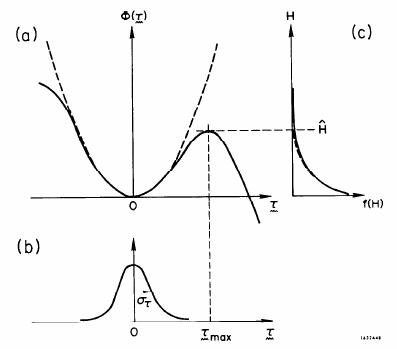
\includegraphics[width=0.8\linewidth]{./Figuras/fig48.jpeg}
	\caption{Quantum spread in the energy oscillations.}
	\label{fig:fig48}
\end{figure}

Suppose we let $H$ represent the ``total oscillation energy'' -- that is, the sum of the ``potential
 energy'' and the ``kinetic energy'' of Eq.~\eqref{eq:5.131} --
\begin{align}
	H = \Phi(\tau) + \dfrac{\alpha^2}{2} \left( \dfrac{\epsilon}{E_0} \right)^2,
\end{align}
($\Phi$ is taken to be zero at the bottom of the potential well) During the oscillation of any particular electron the ``potential energy'' reached at the maximum of $\tau$ is equal to $H$. And the peak ``kinetic energy'' -- which occurs as the electron passes $\tau = 0$ -- is also equal to %
$H$, so
\begin{align}
	H = \dfrac{\alpha^2}{2} \dfrac{\hat{\epsilon}^2}{E_0^2}.
\end{align}
where $\hat{\epsilon}$ is the peak value of $\epsilon$ during its oscillation. An electron is captured in a stable energy oscillation if $H$ is less than $\Phi_\text{max}$, the maximum height of the potential well (See Section~\ref{sec:3.6}). Otherwise it will be lost.\\
In Sections~\ref{sec:5.2} and \ref{sec:5.3} we have examined the quantum-induced energy oscillations under the assumption that they were ideally linear -- which would correspond to the ideal parabolic potential-well indicated by the broken line in Fig.~\ref{fig:fig48}(a). Under these assumptions, the distribution of time displacements in a stored bunch of electrons would be as the Gaussian function drawn in Fig.~\ref{fig:fig48}(b) - whose standard deviation $\sigma_\tau$ was evaluated in Section~\ref{sec:5.4}.\\
We have also seen that the energy fluctuations yield an exponential distribution in the square of the amplitude of the energy oscillations -- as described by Eq.~\eqref{eq:5.62}. The quantity $W$ used there is just the square of the amplitude (of the oscillation in $\epsilon$) and is therefore, proportional to the ``total energy'' $H$. In fact,
\begin{align}
	H = \dfrac{\alpha^2}{2 E_0^2}W.
\end{align}
It follows that the distribution over $H$ for the electrons stored in a bunch is also exponential. Specifically, if we let $f(H)dH$ represent the number of electrons with ``total oscillation energies'' between $H$ and $H + dH$, then a direct translation of Eq.~\eqref{eq:5.62} gives
\begin{align}
	f(H)dH = \dfrac{N}{\mean{H}} \exp \left( -H/\mean{H} \right),
\end{align}
where
\begin{align}
	\mean{H} = \dfrac{\alpha^2}{2 E_0^2} \mean{W} = \dfrac{\alpha^2}{E_0^2} \sigma_\epsilon^2.
\end{align}
This distribution in oscillation energies is shown in Fig.~\ref{fig:fig48}(c).\\
The real situation must evidently be different. Any electron whose time displacement once exceeds $\tau_\text{max}$, the value of $\tau$ at the top of the actual potential hill -- or equivalently, one whose ``oscillation energy'' $H$ exceeds $\Phi_\text{max}$ -- will be lost from the stored bunch. As we saw in the preceding section for the radial oscillations, we must expect that the actual distributions will fall to zero at $\tau_\text{max}$ -- and therefore at $H = \hat{H} = \Phi_\text{max}$. And there will be a continuous loss of electrons due to diffusion
 out of the tail of the distribution.\\
The situation here is similar to the one discussed in the preceding section, which would correspond to a parabolic potential well which is suddenly truncated at $\tau_\text{max}$. The smooth rounding of the potential maximum will have a somewhat different effect on the comportment of the distribution of electrons near the edge of the distribution. One may expect however, that so long as $\tau_\text{max} >> \sigma_\tau$, the rate of loss of electrons may be estimated in the same way for both situations.\\
Without repeating the argument here, we may write the result which corresponds to Eq.~\eqref{eq:5.127}, translated to the case of the energy oscillations,
\begin{align}
	\tau_q = \dfrac{\tau_\epsilon}{2} \dfrac{e^\xi}{\xi},
\end{align}
with
\begin{align}
	\xi = \dfrac{\hat{H}}{\mean{H}} = \dfrac{\Phi_\text{max}}{\mean{H}}.
\end{align}
The height $\Phi_\text{max}$ of the potential maximum can be evaluated by performing the integration of Eq.~\eqref{eq:3.53} -- or for a sinusoidal rf voltage, from Eq.~\eqref{eq:3.58}.\\
The potential $\Phi_\text{max}$ was introduced in order to obtain the magnitude of the ``aperture''
 of the energy oscillations. It is related to the maximum acceptable energy deviation $\epsilon_\text{max}$ -- see Eq.~\eqref{eq:5.57} --
\begin{align}
	\Phi_\text{max} = \dfrac{\alpha^2}{2} \left( \dfrac{\epsilon_\text{max}}{E_0} \right)^2.
\end{align}
So $\xi$ has the conceptually simple form
\begin{align}
	\xi = \dfrac{\epsilon_\text{max}^2}{2\sigma_\epsilon^2}.
\end{align}
The potential $\Phi_\text{max}$ and, therefore, the number $\xi$ depends on the magnitude of the rf voltage which must always be sufficiently large to give a quantum lifetime greater than the desired storage time of the beam. Typically $\xi$ must be at least as large as 18 or so, requiring that $\epsilon_\text{max}/\sigma_\epsilon$ be about 6.\\
For the particular (but very common) case of a storage ring with an isomagnetic guide field and a sinusoidally varying rf voltage, the parameter $\xi$ can be expressed rather simply in terms of the ring parameters. Bringing together the results obtained in earlier sections for $(\epsilon_\text{max}/E_0^2) = \frac{U_0 F(q)}{\pi \alpha k E_0}$ and $(\sigma_\epsilon/E_0)^2 = \frac{C_q\gamma_0^2}{J_\epsilon \rho_0}$ you can show that
\begin{align}
	\xi = \dfrac{J_\epsilon E_0}{\alpha k E_1} F(q) && \text{(isomag.)}.
\end{align}
where $E_1$ is a constant with the dimensions of an energy:
\begin{align}
	E_1 = \dfrac{3mc^2 C_q}{2 r_e} = \dfrac{55 \sqrt{3}}{64} \dfrac{\hslash c}{r_e} \approx 1.08 \times 10^8 \text{eV},
\end{align}

since $U_0 = \frac{C_\gamma E_0^4}{\rho_0}$ for isomagnetic guide fields and $C_\gamma = \frac{4\pi r_e}{(mc^2)^3}$. $F(q)$ is the energy aperture function which was defined in Eq.~\eqref{eq:3.60} and is shown in Fig.~\ref{fig:fig38}. The parameter $q$ is the rf overvoltage -- namely the ratio of the peak rf voltage to the energy lost in one turn. For large overvoltages $F(q)$ is approximately $(2q- \pi)$ and the quantum lifetime increases exponentially with increasing rf voltage.\\
Notice that in a storage ring with a given guide field (that is with a fixed $\alpha$,
$J_\epsilon$, $\tau_\epsilon$ and $E_0$) the overvoltage required for any particular quantum lifetime (that is for a particular $\xi$) depends on the harmonic number $k$ of the rf system. For large harmonic numbers the overvoltage required varied approximately as $\sqrt{k}$.
